% arara: pdflatex

\documentclass[a4paper, 12pt]{report}

%-----------------------------------------------------------------------------
% Packages
%-----------------------------------------------------------------------------
\usepackage[T1]{fontenc}            % Font encoding
\usepackage[utf8]{inputenc}         % Input encoding
\usepackage[english,italian]{babel} % Text Language (secondaria, primaria)
\usepackage{microtype}              % Improves text writing
\usepackage{graphicx}               % Required for inserting images
\usepackage{subfig}
\usepackage{caption}
\usepackage{float}                  % For figures
\usepackage{hyperref}
\hypersetup{
    colorlinks=true, 
    linkcolor=blue,
    urlcolor=blue,
    pdfstartview = XYZ null null 1.00,  % open the generated pdf with 100% zoom by default, 
    pdftitle={IPA Project presentation},
}

% Set the custom path for images
\graphicspath{{./images/}}


\begin{document}


%\begin{titlepage}

    \thispagestyle{empty}




    \begin{center}
        \normalsize{UNIVERSITÀ DEGLI STUDI DI \\ CASSINO E DEL LAZIO MERIDIONALE}
    \end{center}
    
    
    
    \begin{figure}[!htp]
        \centering
        \includegraphics[keepaspectratio=true,scale=0.1]{./Unicas_logo.pdf}
    \end{figure}
    
    
    \begin{center}
        \Large{IPA PROJECT PROPOSAL}
    \end{center}
    
    
    \vspace{7mm}
    
    
    \begin{center}
        \LARGE{\textbf{Aircraft detection from satellite images}}
    \end{center}
    
    
    
    \begin{figure}[!htp]
        \centering
        \includegraphics[keepaspectratio=true,scale=0.6]{./satellite_aircraft_detection.png}
    \end{figure}
    
    \vspace{10mm}
    
    
    \begin{minipage}[t]{0.47\textwidth}
        {\normalsize{\textbf{Docente:}}{\normalsize\vspace{3mm}
        \\ \large{Prof. Alessandro Bria}}}
    \end{minipage}
    \hfill
    \begin{minipage}[t]{0.47\textwidth}\raggedleft
        {\normalsize{\textbf{Gruppo:}}{\normalsize\vspace{3mm} 
            \\ \large{Giuseppe Alfieri \\
                      Riccardo D'Aguanno \\
                      Gianmarco Luongo \\
                      Aurora Pisa \\
                      Paolo Simeone}}}
    \end{minipage}
    
    
    \vspace{10mm}
    
    
    {\centering{\large{ANNO ACCADEMICO 2023/2024}}\par}
    
    %\end{titlepage}
    


\section*{Considerazioni preliminari}


Stante la numerosità del \emph{dataset} \href{https://github.com/dilsadunsal/HRPlanesv2-Data-Set}{HRPlanesv2} (Figura~\ref{fig:dataset_info}) abbiamo, preliminarmente, ridotto lo stesso
di un ordine di grandezza (splittando, con l'ausilio di uno script \emph{bash}, le $1490$ immagini in cinque blocchi da $298$ e delegando ad ogni membro del gruppo l'onere di sceglierne $10$ da ogni blocco) perseguendo l'eterogeneità delle immagini secondo criteri quali:

\begin{itemize}
    \item condizioni atmosferiche 
    \item[] % elemento vuoto per separare il testo dall'immagine
        \begin{minipage}[t]{\linewidth}
            \centering
            \includegraphics[width=0.4\linewidth]{./488_DT8.png}
            \quad % spazio tra le immagini se necessario
            \includegraphics[width=0.4\linewidth]{./226_DT8.png}
        \end{minipage}
    \item coesistenza di diverse tipologie di aerei (civili/militari) nella medesima immagine
    \item[] % elemento vuoto per separare il testo dall'immagine
        \begin{minipage}[t]{\linewidth}
            \centering
            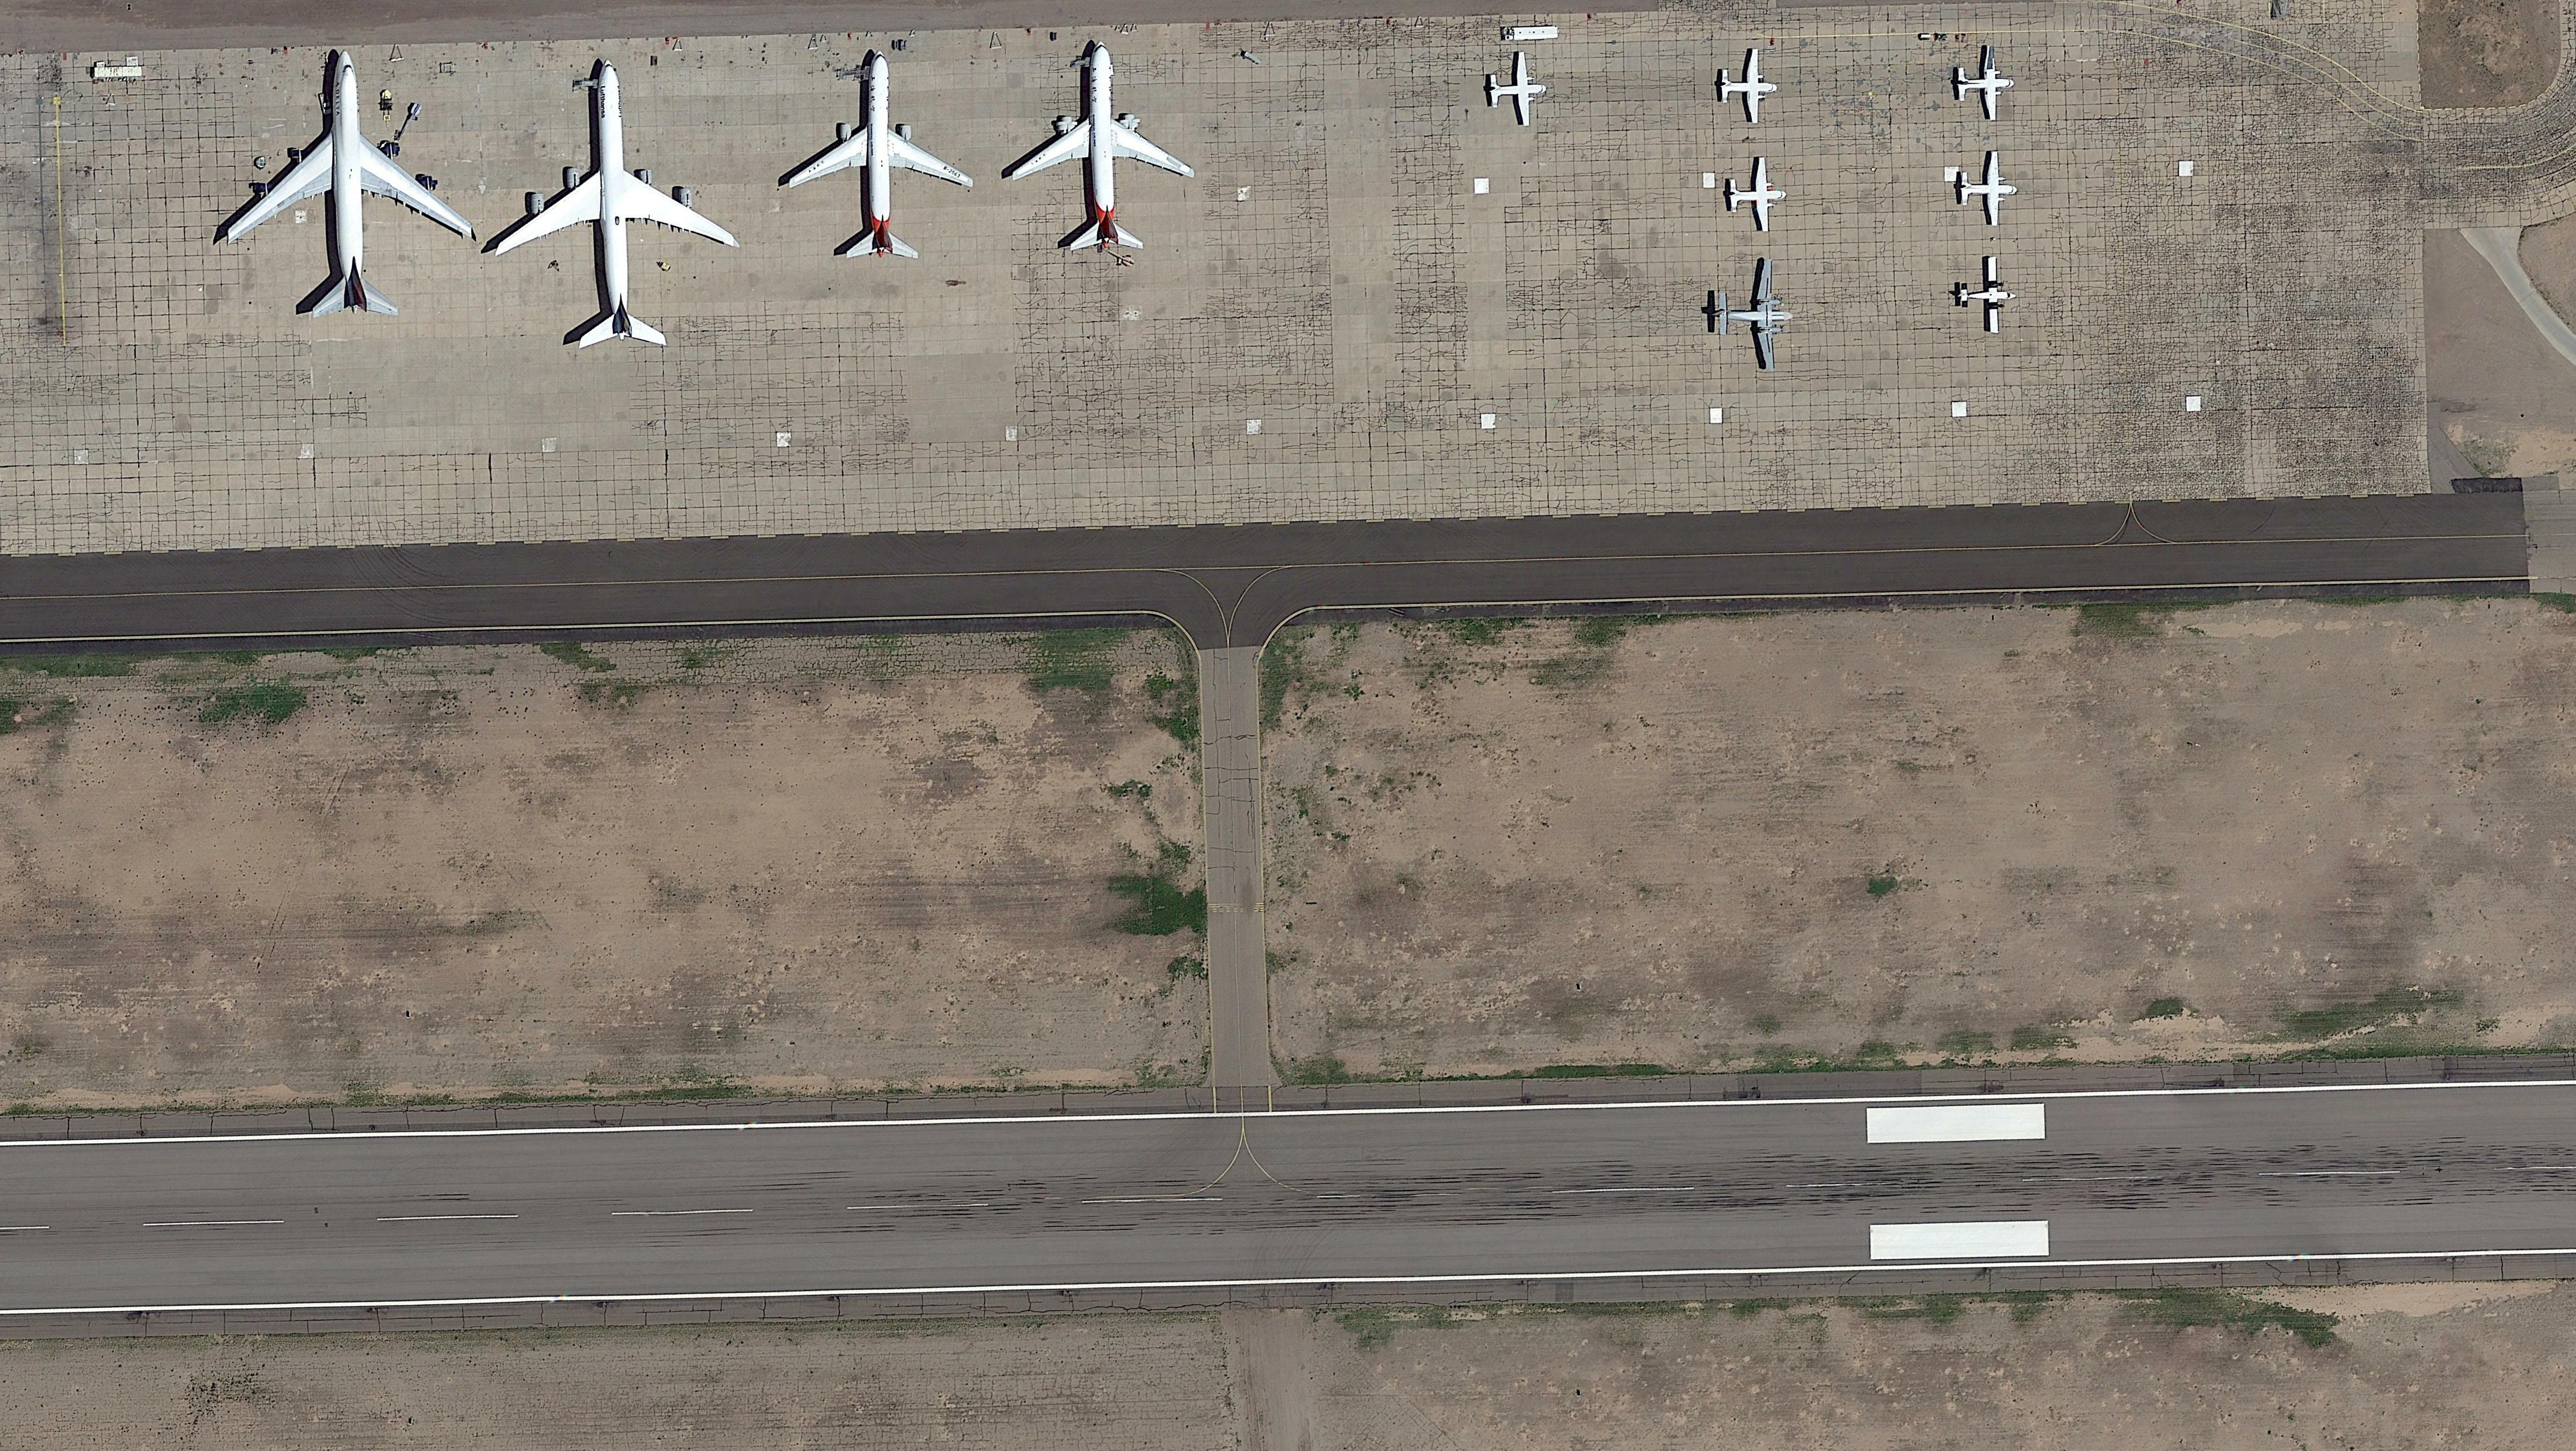
\includegraphics[width=0.4\linewidth]{./1_DT4.png}
        \end{minipage}
\end{itemize}

\begin{figure}
   \centering
   \includegraphics[keepaspectratio=true,scale=0.6]{./dataset_info.png}
    \caption{Composizione del dataset}
    \label{fig:dataset_info}
\end{figure}



\section*{Task}

Rilevamento di aerei da immagini satellitari.



\end{document}
